\section{Case Studies}

We present two example applications in RCloud based on synthetic data
and applications.\footnote{Unfortunately, we could not show production
notebooks that may contain proprietary or confidential information.}
The main point of the examples is to show key steps in the visual
analytics development and deployment process that we aimed to support.

\subsection{Stock Price Analysis\label{sec:stockvis}}

\begin{figure}
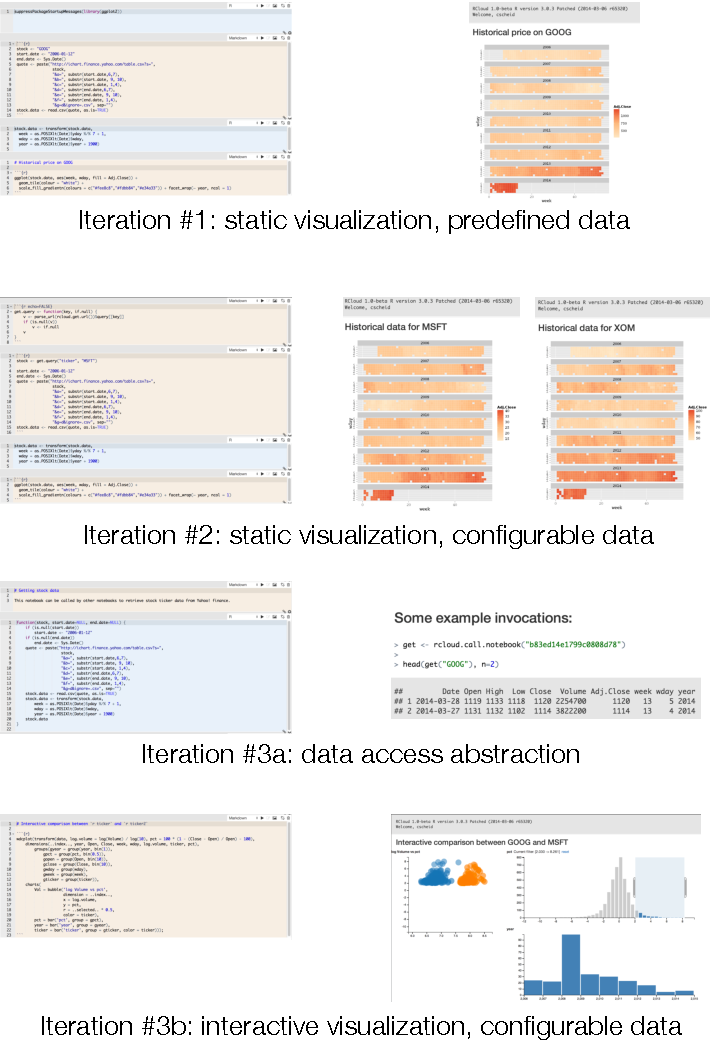
\includegraphics[width=\linewidth]{fig/casestudy1/casestudy1.pdf}
\caption{\label{sec:stockvis}Iterations of a stock ticker
  visualization, based on an example by Hadley Wickham. A
  simple, static visualization of the closing price of a single stock
  is progressively developed into a configurable display suitable
  for dashboarding, then into an interactive visualization for 
  comparing the volatility and volume of two stocks, and finally
  into an API for data access by other RCloud notebooks. The notebooks
  in this example can all be loaded as web pages. When a notebook
  corresponding to a function call is displayed a web page,
  its associated documentation is displayed.}
\end{figure}

Our first example is a sequence of visualizations of the performance
of financial stocks over a multi-year period. The first visualization
in this example uses ggplot2 and is due to Hadley Wickham. It reads
data provided by Yahoo! Finance as a web service, and shows the price
for a single trading symbol.

The webpage that produces that visualization includes a link back to
the generating source code, from which a user can fork the notebook
and, in this case, add a configurable ticker based on the URL of
the notebook. Notice that the notebook changes very little.

From there, the notebook author or a collaborator may decide to
provide convenient access to the data, apart from its visualization.
This is done by creating a notebook that defines a function.
That notebook then becomes a \emph{subroutine} for other notebooks,
and is version-controlled like other notebooks.

\todo{Interactive version.}

%% This notebook can then be called in an \emph{interactive}
%% visualization, which uses the Javascript 

%% Easy to convert it into configurable entry point for dashboarding.

%% Now consider an analyst that wants to understand the price dynamics of
%% different stock attributes, different points in time, etc. For that,
%% interactive visualization is very attractive. describe dcplot and
%% notebook which uses it.

%% Then describe abstraction of stock-data fetching, to talk about
%% calling notebooks from other notebooks.

%% then call.r?

\subsection{text analysis\ref{sec:textvis}}

Same.

% IMPORTANT: what is unique about RCloud here
% From prototyping to dashboard
% Getting other information from the web
%
